\section{Kravspecifikation}

\subsection{General beskrivelse}
\begin{table}[H]
    \begin{minipage}{.6\textwidth}
        \begin{figure}[H]
            \centering
            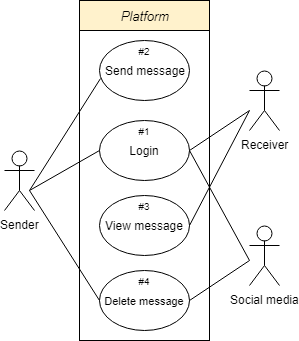
\includegraphics[width=0.70\linewidth]{Projectdoc/Assets/Illustrationer/simple-usecase.png}
            \caption{Usecase diagram}
            \label{fig:usecase}
        \end{figure}
    \end{minipage}
    \begin{minipage}{.4\textwidth}
        Det endelige system er en meddelelsesplatform, sikkert med en form af steganografi. Brugerne skal kunne logge ind i systemet, hvor brugeren derefter har adgang til at sende og modtage information. Følgende use-case forløb beskriver grundelementerne i meddelelsesplatformen.
        \\\\
        Given denne overstående beskrivelse, kan der i alt formuleres to forskellige hovedscenarier for produktets anvendelse, der begge definerer produktets endelige mål.
    \end{minipage}
\end{table}

\subsection{Udvidet beskrivelse}
\subsubsection{Usecase: Send besked}
\label{Hovedscenarie1}
For forsendelse, af beskeder gennem produktet, vil brugeren skulle først udføre usecase \#1. "Login" [\ref{Usecase1_Login}]. Denne usecase vil registre brugeren til senere genkendelse, for f.eks. muligheden til redigering, eller at slette deres oprettede besked tråde, eller enkelte posts. Brugeren kan dog også vælge at foretage en såkaldt anonym registration, hvor brugren ikke selv direkte sættes i sammenhæng med den postede besked, men i stedet er blevet formidlet igennem en fælles talsperson registreret af produktet selv. Efterfølgende vil brugeren skulle udføre usecase \#2. "Send message" [\ref{Usecase2_Send_Message}], hvor brugeren blandt andet vil få mulighed for at vælge f.eks. en specifik sammenhæng, hvori brugerens besked vil blive kædet sammen. Det bagved læggende system vil efterfølgende håndtere kryptering af beskedens tekst, og dens indarbejdelse i en steganografisk sammenhæng, og vil efterfølgende også gennem API strukturer, udgive den nedskrevne besked til det aktuelle sociale medie. For uddybende beskrivelse se appendix: [\ref{Usecase2_Send_Message}]
\newpage

\subsubsection{Usecase: Se beskeder}
\label{Hovedscenarie2}
For fremvisning af beskeder i produktet, vil brugeren som i forgående hovedscenarie [\ref{Hovedscenarie1}] først skulle udføre usecase \#1. "Login". Efter denne skal brugeren gennemgå usecase \#3 "View message" [\ref{Usecase3_View_Message}], hvor brugeren vil blive præsenteret med muligheden for at vælge, først en specifik tråd, hvori der kan forekomme en række af flere enkelte beskeder, og efterfølgende f.eks. en længere enkelt stående tekst besked.
Selvfølgelig er denne omtalte tråd og tekst repræsentation ikke fremvist under steganografi, men er blevet bearbejdet af systemet til igen at være læselig for brugeren ved tilgang.
Endvidere under disse fremvisninger, kan en bruger også vælge, at slette en besked eller hele tråde, såfremt at brugeren har registreret ejerskab over disse. For uddybende beskrivelse se appendix: [\ref{Usecase3_View_Message}]

\subsection{Krav til produktet}
\textit{Systemet indeholder: Kommunikationsplatformen og dens servere}
\begin{enumerate}[label=\textbf{Krav \arabic*},leftmargin=.80in]

    \item \label{k:send} Systemet skal kunne sende beskeder/indlæg.
    \item \label{k:vise} Systemet skal kunne vise beskeder/indlæg.
    \item \label{k:lagre} Beskeder skal lagres på et socialt medie.
    \item \label{k:stegano} Lagrede beskeder skal være skjult via steganografi.
    \item \label{k:anonymt} Systemet skal foretage kommunikationen anonymt.
    \item \label{k:indstil} Der må ikke forekomme indstillinger der påvirker brugernes sikkerhed.

    \item \label{k:slette} Brugere skal kunne slette tidligere sendte beskeder.
    \item \label{k:sammen} Beskeder skal kunne kædes i længere sammenhæng.
    \item \label{k:naviger} 80\% af testbrugerne skal kunne navigere systemet uden yderligere instruktioner.
    \item \label{k:sikker} Det skal være tydeligt for mindst 80\% af testbrugerne, at deres kommunikation er sikker.
    \item \label{k:krypto} Systemet må ikke udelukkende sikres med steganografi.
    \item \label{k:load} Systemet må ikke tage mere end 10 sekunder om at indlæse en indlægsoversigt.
\end{enumerate}